\documentclass[10pt]{article}

\usepackage{graphicx}
\usepackage[export]{adjustbox}
\usepackage[paperwidth=6in, paperheight=7.5in]{geometry}
\geometry{left=0cm,right=0cm, top=0cm,bottom=0cm}
\usepackage{stackengine} % for labels (A) (B).. on subfigures
\usepackage{hyperref}

% label style
\newcommand\bsf[1]{\Large{\textbf{\textsf{#1}}}}

\begin{document}

%-----------------------------------------------------------------------
\begin{figure}
    \centering
    \stackinset{l}{0in}{t}{0in}{\bsf{A}}{
        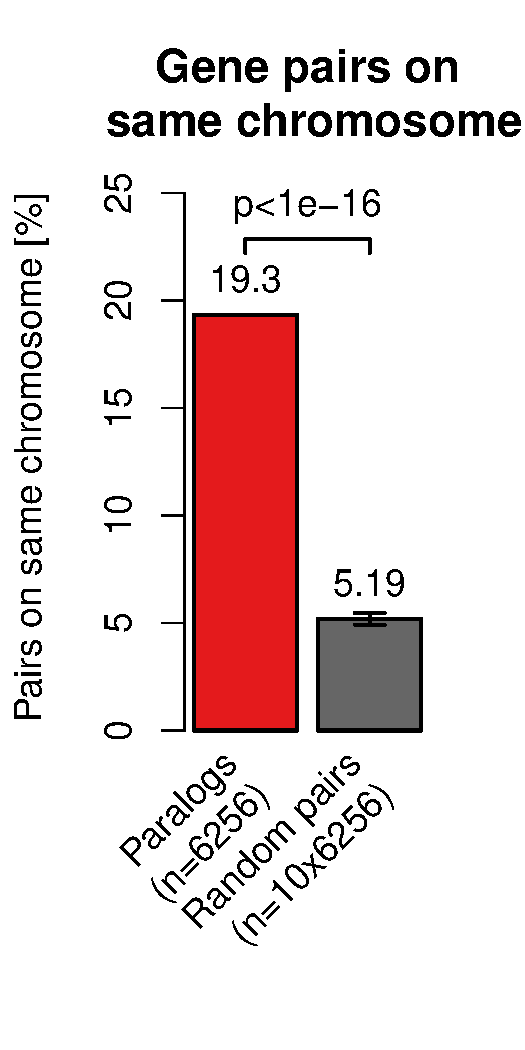
\includegraphics[width=.19\columnwidth]{{select_old_pairs/EnsemblGRCh37_paralog_genes.paralogPairs_on_same_chrom.barplot}.pdf}
    }\stackinset{l}{0in}{t}{0in}{\bsf{B}}{
        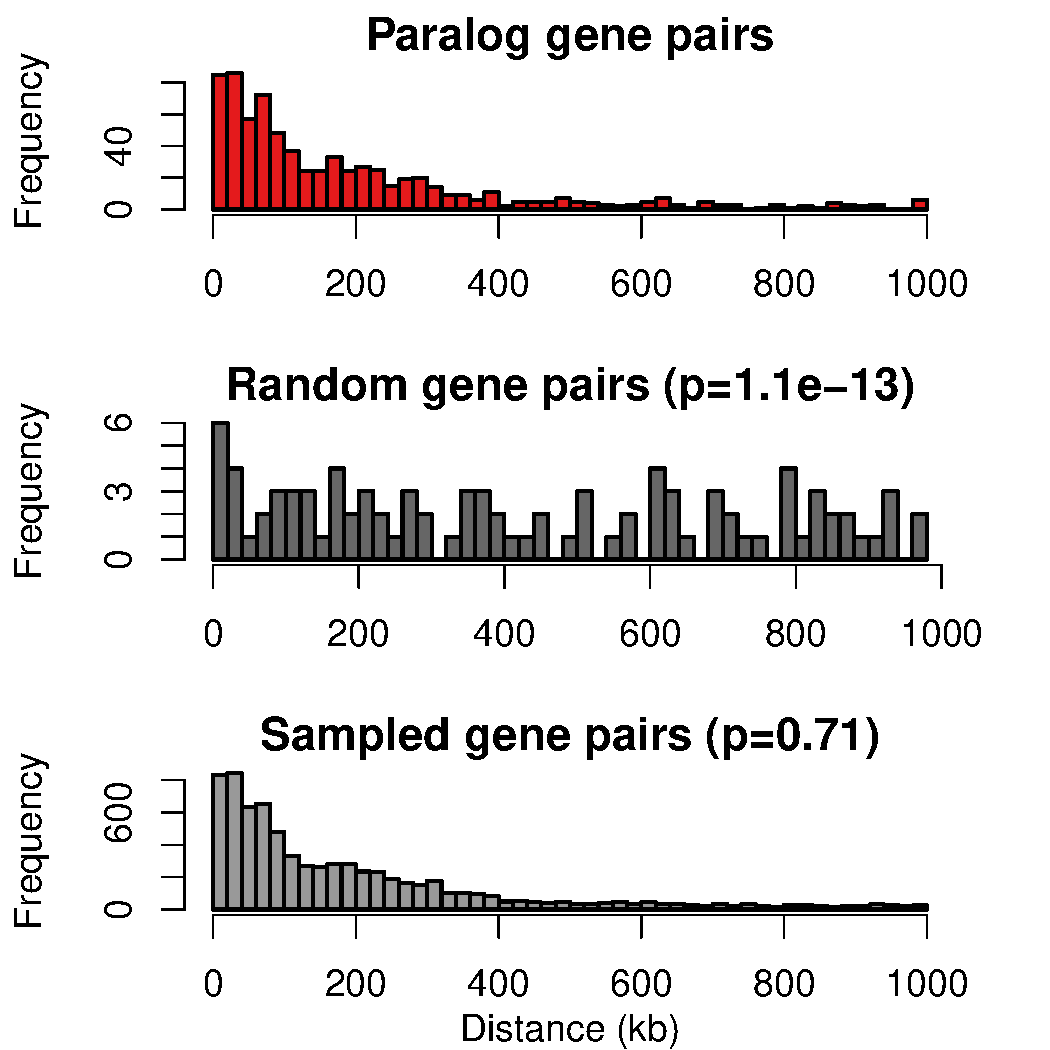
\includegraphics[width=.38\columnwidth]{{select_old_pairs/EnsemblGRCh37_paralog_genes.samped_random_para_dist.hist}.pdf}
    }\stackinset{l}{0in}{t}{0in}{\bsf{C}}{
        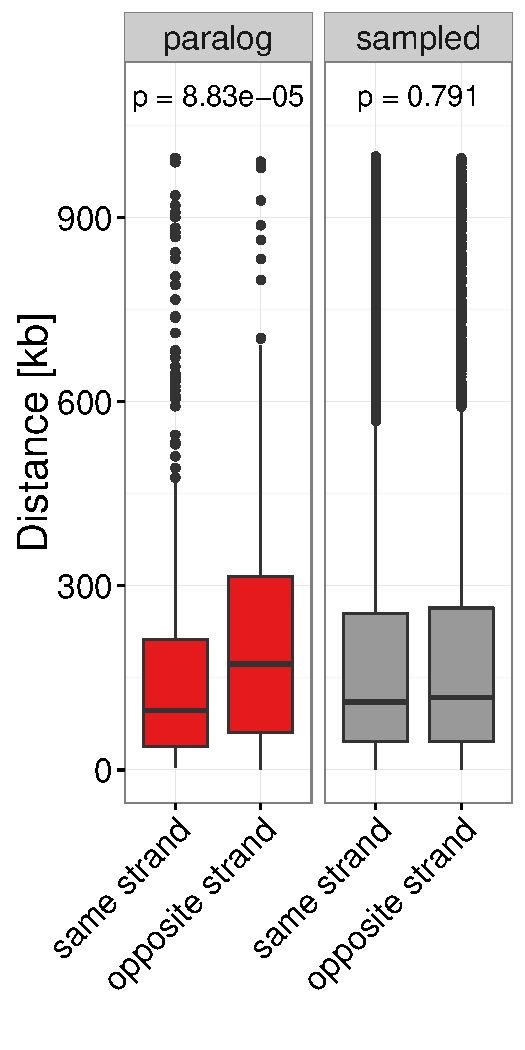
\includegraphics[width=.19\columnwidth]{{select_old_pairs/EnsemblGRCh37_paralog_genes.close.dist_by_sameStrand_and_group.boxplot}.pdf}
    }\stackinset{l}{0in}{t}{0in}{\bsf{D}}{
        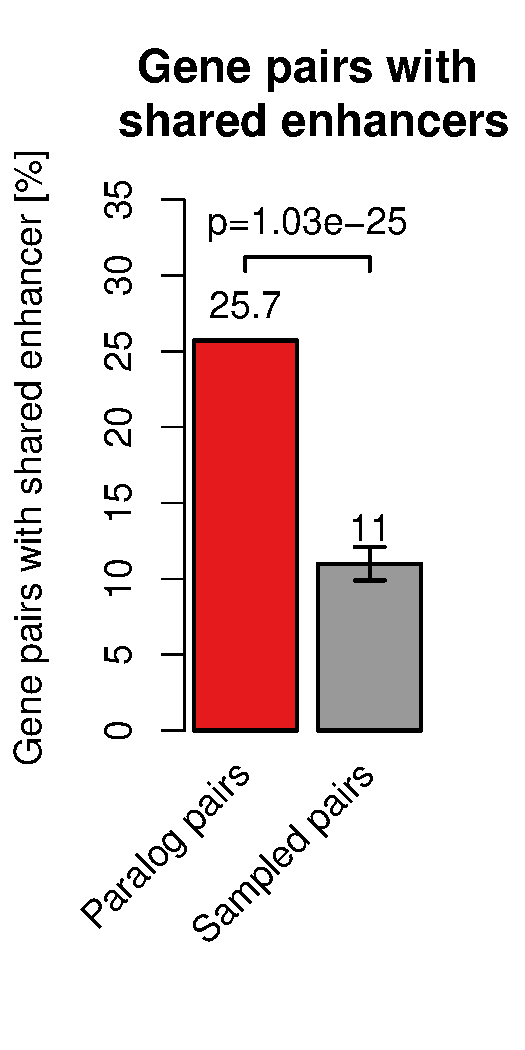
\includegraphics[width=.19\columnwidth]{{select_old_pairs/EnsemblGRCh37_paralog_genes.paralogPairs.has_shared_enhancer.barplot}.pdf}}

    \stackinset{l}{0in}{t}{0in}{\bsf{E}}{
        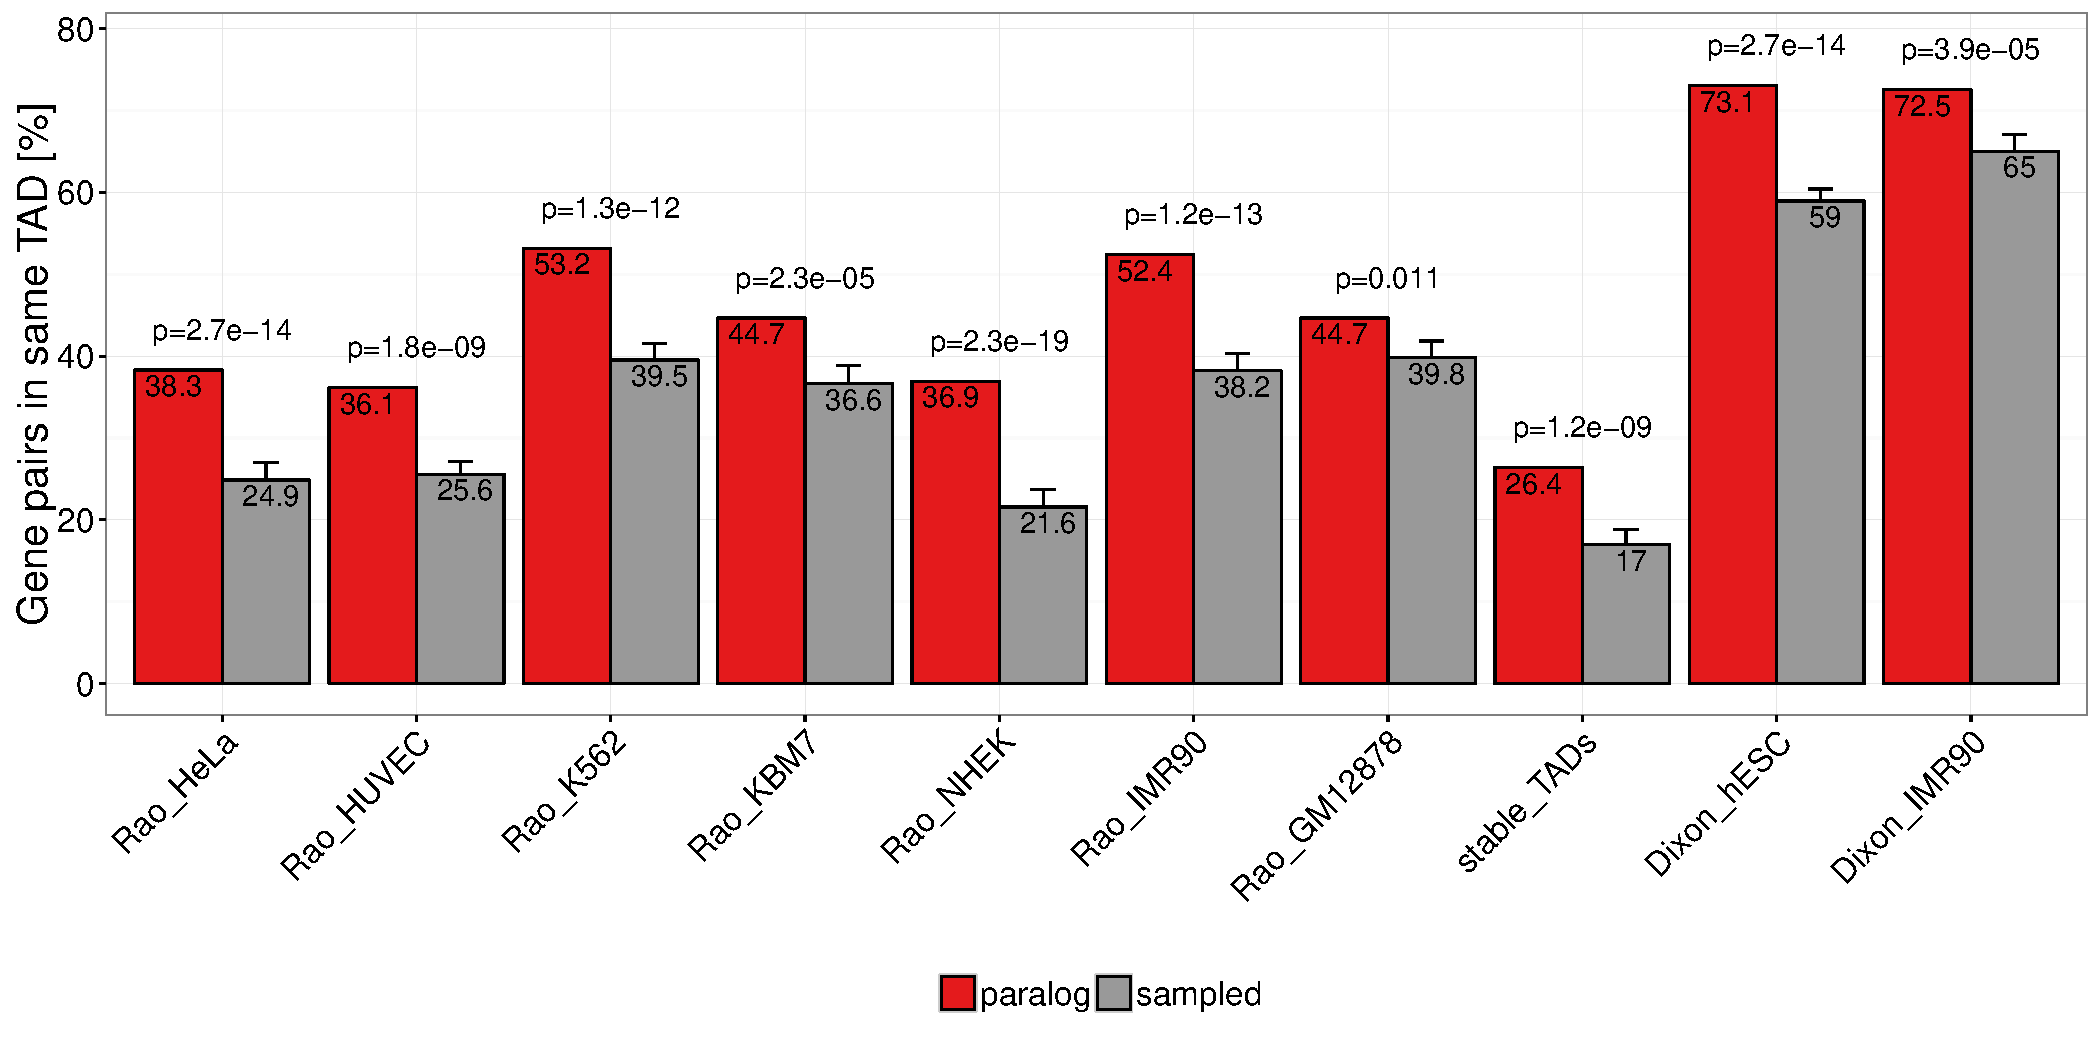
\includegraphics[width=.95\textwidth]{{select_old_pairs/EnsemblGRCh37_paralog_genes.close.percent_gene_pairs.by_group_in_TAD_TADsource.barplot}.pdf}
    }

    \stackinset{l}{0in}{t}{0in}{\bsf{F}}{
        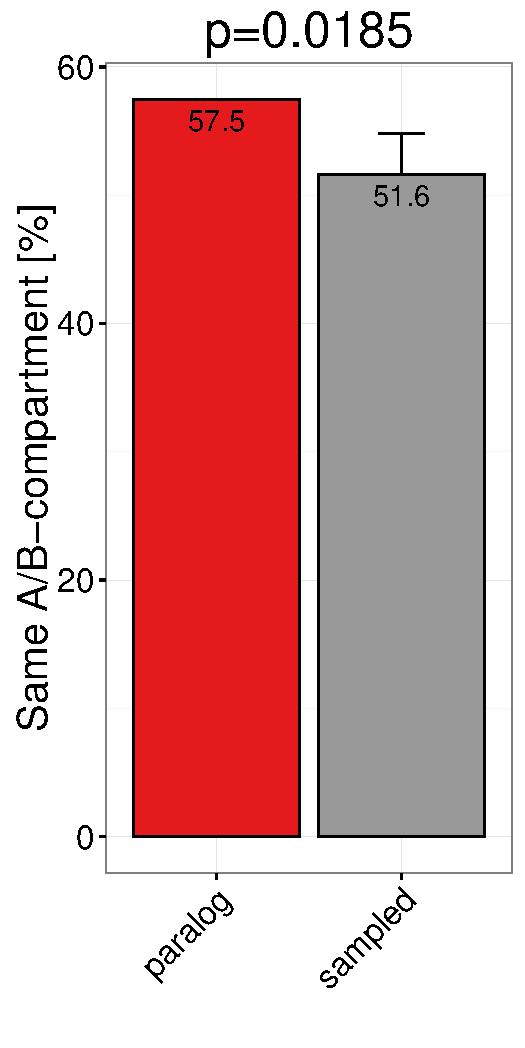
\includegraphics[width=.2\textwidth]{{select_old_pairs/EnsemblGRCh37_paralog_genes.common_compartment}.pdf}
    }
    \stackinset{l}{0in}{t}{0in}{\bsf{G}}{
        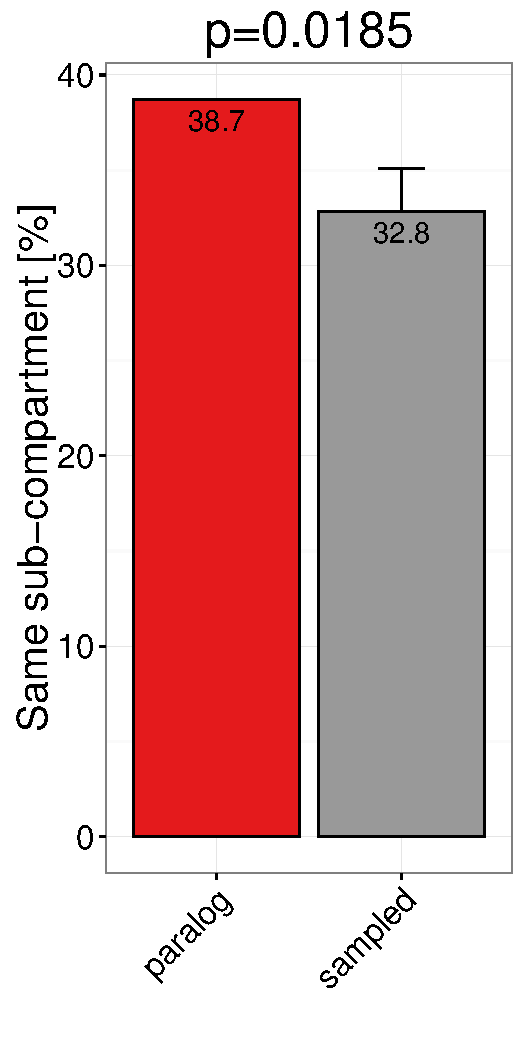
\includegraphics[width=.2\textwidth]{{select_old_pairs/EnsemblGRCh37_paralog_genes.common_subcompartment}.pdf}
    }
    \stackinset{l}{0in}{t}{0in}{\bsf{H}}{
        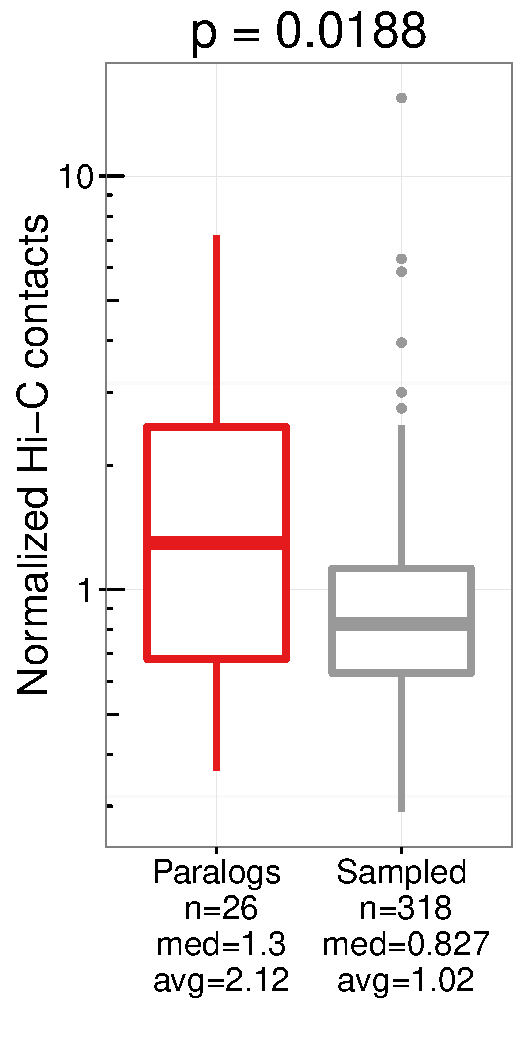
\includegraphics[width=.2\textwidth]{{select_old_pairs/EnsemblGRCh37_paralog_genes.distal.HiCNoZero.ggboxplot}.pdf}
    }
    \stackinset{l}{0in}{t}{0in}{\bsf{I}}{
        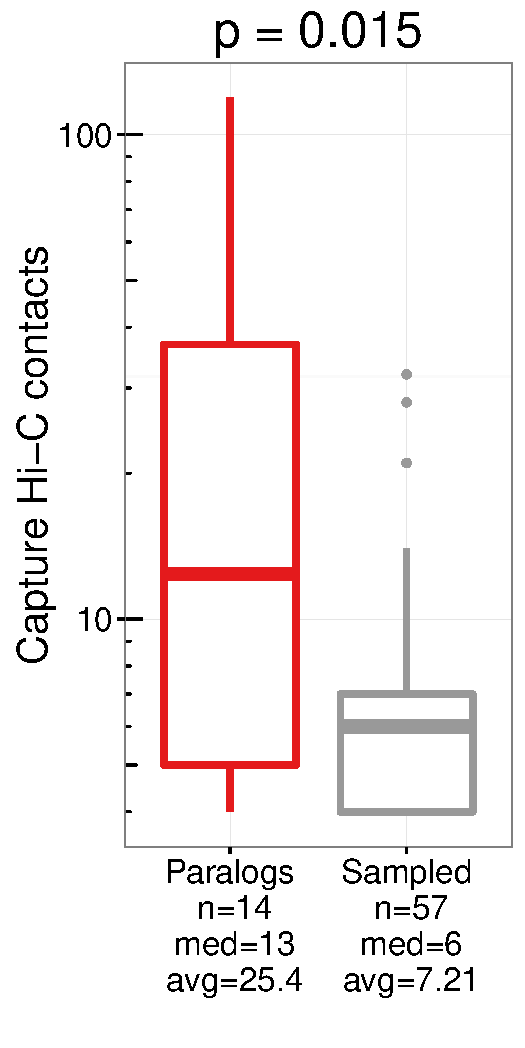
\includegraphics[width=.2\textwidth]{{select_old_pairs/EnsemblGRCh37_paralog_genes.distal.captureC_rawNoZero.ggboxplot}.pdf}
    }
%~ \caption{
%~ }
%~ \stackinset{r}{0cm}{b}{0cm}{\textbf{Fig. 3}}{\makebox[\textwidth]{~}}
\end{figure}


%-----------------------------------------------------------------------
\end{document}


